% Justification du guide générique de CT-CORA3D (projet PMD2, ECAM)
% Compilateur Overleaf : pdfLaTeX.
\documentclass[11pt,a4paper]{article}

\usepackage[utf8]{inputenc}
\usepackage[T1]{fontenc}
\usepackage[french]{babel}
\frenchsetup{StandardItemLabels=true, CustomiseFigTabCaptions=false}
\usepackage{lmodern}
\usepackage{newunicodechar} % lettres grecques tapées directement dans le texte
\newunicodechar{α}{\ensuremath{\alpha}}
\newunicodechar{δ}{\ensuremath{\delta}}
\newunicodechar{Ø}{\O}
\usepackage[margin=2.3cm]{geometry}
\usepackage{graphicx}
\usepackage[labelsep=colon]{caption}
\addto\captionsfrench{\renewcommand{\tablename}{Tableau}}
\usepackage{xcolor}
\usepackage{tabularx}
\usepackage{booktabs}
\usepackage{longtable}
\usepackage{enumitem}
\usepackage{fancyhdr}
\usepackage{titlesec}
\usepackage[hidelinks]{hyperref}

\hyphenpenalty=10000
\exhyphenpenalty=10000
\emergencystretch=3em

\definecolor{ecam}{RGB}{30,60,140}
\titleformat{\section}{\Large\bfseries\color{ecam}}{\thesection.}{0.6em}{}
\titleformat{\subsection}{\large\bfseries\color{ecam}}{\thesubsection}{0.6em}{}
\setlist{itemsep=2pt}
\setlength{\parindent}{0pt}
\setlength{\parskip}{0.6em plus 0.2em}
\renewcommand{\arraystretch}{1.2}

\pagestyle{fancy}
\fancyhf{}
\lhead{\small Justification du guide générique}
\rhead{\small CT-CORA3D, projet PMD2, ECAM}
\cfoot{\thepage}

\newcommand{\echelle}{{\NoAutoSpacing 2:1}}

\begin{document}

\begin{center}
  
\includegraphics[width=0.22\textwidth]{images/logo_ecam.png}\par\vspace{0.4cm}
  {\LARGE\bfseries\color{ecam} Justification du guide générique\par}\vspace{0.2cm}
  {\large CT-CORA3D : guide de coupe et guide de réduction\par}\vspace{0.3cm}
  {\normalsize Dorian Verstappen, Imane Bikass, Mohamed-Amine Ahmidouch\par}
  {\normalsize Master en ingénierie biomédicale, ECAM Brussels Engineering School, \today\par}
\end{center}

\section{La question}

Le logiciel CT-CORA3D construit, pour chaque chien, un guide de coupe et un guide de réduction imprimables. Tous ces
guides sont dérivés d'un même modèle, le \textbf{guide générique}. Ce rapport explique sur quoi ce modèle repose,
de quoi il est fait, comment ses dimensions ont été choisies et sur quel os il est dessiné.

\section{Réponse courte}

\begin{itemize}
  \item Le guide générique \textbf{ne repose sur aucun os en particulier}. C'est un modèle paramétrique : une liste de
        dimensions de conception (épaisseurs, jeux, hauteurs) qui ne dépendent pas de l'animal.
  \item Pour le dessiner (plans CTC3D-GEN-01 et CTC3D-GEN-02), nous utilisons un \textbf{os cylindrique nominal de
        16~mm de largeur}, qui n'est pas représenté sur les plans. Ce n'est donc pas l'os fictif.
  \item L'\textbf{os fictif} (modèle 3D d'un fémur et d'un tibia, généré par le programme) sert à autre chose : tester
        la planification et la construction des guides sur un os dont tous les repères sont connus exactement.
  \item Pour un vrai chien, le logiciel reprend le modèle générique et l'adapte à l'os segmenté sur le scanner : la
        coque est moulée sur l'os et les dimensions qui dépendent de l'os sont recalculées.
\end{itemize}

\section{Les trois os du projet et leur rôle}

\begin{tabularx}{\textwidth}{@{}lXl@{}}
\toprule
\textbf{Os} & \textbf{Rôle} & \textbf{Utilisé pour} \\ \midrule
Os nominal (cylindre de 16~mm) & support du dessin du modèle générique, sans anatomie & plans 2D génériques \\
Os fictif (modèle 3D) & os connu exactement, déformé à volonté & tests, démonstrations \\
Os du lévrier (scanner) & os réel segmenté & validation sur un cas réel \\
\bottomrule
\end{tabularx}

\paragraph{L'os fictif.} Il est généré par le programme \texttt{generate\_bones.py} : fémur, tibia, fibula, rotule et
fabelles d'un membre pelvien droit de chien de type Labrador d'environ 30~kg. Les formes sont construites à partir de
volumes simples (sphères, ellipsoïdes, tubes) assemblés sans arête vive. Le modèle sain est calibré sur les angles
publiés : aLPFA 103° et aLDFA 97° pour le fémur (Tomlinson 2007), mMPTA 93,4° et mMDTA 96,3° pour le tibia (Dismukes
2007), mCaPTA 63,8° et mCrDTA 81,7° (Dismukes 2008). Comme chaque repère anatomique est connu exactement, on peut
lui appliquer une déformation connue et vérifier que le logiciel la retrouve et la corrige.

\paragraph{Pourquoi pas l'os fictif pour le plan générique ?} Un plan générique doit montrer la \textbf{logique} du
guide : chaque cote y est écrite avec son paramètre, par exemple « 18 (l + 2) » pour la longueur de la fente. Sur un
os réel ou fictif, la coque suit les reliefs de l'os et les cotes changent d'une coupe à l'autre ; le modèle ne serait
plus lisible. Le cylindre donne des sections simples, où chaque dimension se lit directement.

\paragraph{Pourquoi 16~mm ?} C'est une valeur ronde, du même ordre que la largeur des os du projet au niveau de la
coupe (tableau~\ref{tab:largeurs}). Elle ne change rien aux paramètres du guide : elle ne sert qu'à donner des
nombres au dessin.

\begin{center}
  \captionsetup{type=table}
  \caption{Largeur de l'os au niveau de la coupe, mesurée sur les guides de démonstration (longueur de la fente moins
  2~mm).}
  \label{tab:largeurs}
  \begin{tabularx}{0.82\textwidth}{@{}Xr@{}}
  \toprule
  \textbf{Os et cas} & \textbf{Largeur à la coupe} \\ \midrule
  Os fictif : tibia, coin d'ouverture & 13~mm \\
  Os fictif : tibia, coin de fermeture & 13~mm \\
  Os fictif : fémur, coin de fermeture & 18~mm \\
  Lévrier : fémur, coin de fermeture & 21~mm \\
  Lévrier : tibia, coin de fermeture & 21~mm \\
  \textbf{Os nominal des plans génériques} & \textbf{16~mm} \\
  \bottomrule
  \end{tabularx}
\end{center}

\section{D'où viennent les dimensions du guide}

Chaque dimension par défaut indique sa source dans le fichier \texttt{parametres.py} du logiciel. Il y a trois
sources.

\paragraph{1. Le document Best\_Position (BP), contrat du projet.} Il donne les ordres de grandeur ; nous avons pris
une valeur dans chaque intervalle.

\begin{center}
  \begin{tabularx}{\textwidth}{@{}Xll@{}}
  \toprule
  \textbf{Paramètre} & \textbf{Document BP} & \textbf{Valeur choisie} \\ \midrule
  Jeu entre l'os et la coque (j) & 0,2 à 0,5~mm & 0,3~mm \\
  Épaisseur de la coque (e) & 3 à 4~mm & 3~mm \\
  Épaisseur de la lame de scie (s) & 0,5 à 1~mm & 0,6~mm \\
  Diamètre des broches de Kirschner (\O{}b) & exemple : 1,6~mm & 1,6~mm \\
  \bottomrule
  \end{tabularx}
\end{center}

\paragraph{2. Les guides sur mesure décrits dans les publications vétérinaires.} Le principe général vient de là :
une coque qui épouse l'os, une fente qui tient la lame, des broches qui gardent la correction en mémoire, puis un guide
de réduction qui s'enfile sur les broches. Avec des guides de réduction, les publications rapportent une torsion
corrigée à environ 2° de la cible (Hall 2019 pour le fémur, Jeon 2023 pour le tibia, Bright 2024, De Armond 2022).

\paragraph{3. Nos propres choix, chacun justifié par un calcul ou par la faisabilité.}

\begin{itemize}
  \item \textbf{Hauteur de guidage g = 10~mm} : avec un jeu de fente de 0,2~mm, la lame ne peut s'incliner que de
        atan(0,2 / 10), soit environ 1,1°.
  \item \textbf{Jeu de fente js = 0,2~mm et jeu des manchons jb = 0,2~mm} : valeurs de départ, à régler en
        imprimant des pièces d'essai.
  \item \textbf{Paroi p = 2~mm, épaisseur minimale 1,2~mm} : en dessous, les parois cassent à l'impression en PA12.
  \item \textbf{Dépouille $\delta$ = 5°} : le guide se pose et se retire en ligne droite, sans accrocher l'os.
  \item \textbf{Écart aux os voisins jv = 1~mm et au cartilage mc = 1~mm} : le guide ne repose jamais sur une autre
        surface que l'os à couper.
  \item \textbf{Ponts sécables hp = 5~mm} : ils tiennent les deux moitiés ensemble pendant la pose et se coupent à la
        pince après la coupe de l'os.
  \item \textbf{Broches à kd = 1,2 fois la largeur de l'os de la coupe} : assez loin de la fente pour ne pas fragiliser
        l'os, assez près pour rester dans la diaphyse.
\end{itemize}

\section{De quoi est fait le guide}

Le système comprend \textbf{trois éléments} : le guide de coupe (imprimé), le guide de réduction (imprimé) et deux
broches de Kirschner du commerce. Les deux guides s'impriment en PA12 (frittage laser) ou en résine stérilisable.

\subsection{Le guide de coupe}

Il s'imprime d'une seule pièce, mais il est fait de deux \textbf{moitiés} (proximale et distale) reliées par deux
\textbf{ponts sécables}. Il comprend :

\begin{enumerate}
  \item \textbf{La coque.} C'est la partie qui se pose sur l'os. Sa face intérieure est l'empreinte exacte de la
        surface de l'os, décalée du jeu j = 0,3~mm : le guide ne s'emboîte que dans une seule position. Elle a une
        épaisseur e = 3~mm et couvre l'os sur ± 75° (α) autour de la face d'appui, c'est-à-dire un peu moins de la
        moitié de son tour : assez pour ne pas basculer, assez peu pour se poser par un seul abord. Dans le sens de
        l'os, elle dépasse de m = 8~mm au-delà de chaque broche, et s'arrête à plus de 1~mm (mc) du cartilage
        articulaire.
  \item \textbf{Les tours de fente et les fentes.} Une tour est un mur creux posé sur la coque, dans le plan de coupe.
        La fente qui la traverse a une largeur s + js = 0,6 + 0,2 = 0,8~mm (la lame et un petit jeu) et une longueur
        égale à la largeur de l'os plus 2~mm. Ses parois ont p = 2~mm d'épaisseur : la tour fait donc
        0,8 + 2 × 2 = 4,8~mm d'épaisseur. Son sommet est à j + e + g au-dessus du point le plus haut de l'os dans la
        fente, avec g = 10~mm de guidage minimal. Un coin d'ouverture a une fente ; un coin de fermeture en a deux,
        une par face du coin d'os à retirer. Chaque fente est parallèle à la charnière : la \textbf{profondeur de lame}
        (du sommet de la tour jusqu'à la charnière, ou jusqu'à la corticale opposée en coupe complète) est donc la même
        sur toute la fente ; elle est donnée au chirurgien.
  \item \textbf{Les manchons.} Ce sont deux tubes, un par moitié, qui guident le forage des broches. Trou de
        Øb + jb = 1,6 + 0,2 = 1,8~mm, diamètre extérieur 1,8 + 2 × 2 = 5,8~mm, hauteur environ 13 à 15~mm. La broche
        distale est forée avec l'inverse de la correction : elle n'est pas parallèle à la broche proximale avant la
        correction, et le devient après.
  \item \textbf{Les ponts sécables.} Deux petites colonnes de section p × hp = 2 × 5~mm, aux deux bouts de la première
        fente, en haut de la tour. Ils tiennent les deux moitiés ensemble pendant la pose ; on les coupe à la pince
        après la coupe de l'os, puis chaque moitié se retire en glissant le long de sa broche.
  \item \textbf{Les finitions.} Congés de rayon r = 0,8~mm entre la coque, les tours et les manchons (moins de
        fissures), chanfreins de c = 0,5~mm à l'entrée des fentes et des manchons (la lame et la broche entrent sans
        accrocher), dépouille δ de 5°.
\end{enumerate}

\subsection{Le guide de réduction}

C'est une \textbf{barre} qui porte deux \textbf{manchons parallèles}. Les manchons ont le même trou que ceux du guide de
coupe (1,8~mm), une longueur lr = 12~mm (plus de 6 fois le diamètre de la broche, pour la tenir droite), et leur bout
est moulé sur l'os corrigé, au jeu j près. La barre a une épaisseur tb = 6~mm et reste à au moins er = 4~mm de l'os,
pour laisser la place aux tissus mous et à la plaque. Après la correction, les deux broches sont parallèles : la barre
s'y enfile jusqu'au contact de l'os et tient les deux fragments dans la position planifiée (angle, torsion et
translation) pendant la pose de la plaque.

\subsection{Les broches}

Deux broches de Kirschner de 1,6~mm, une par fragment. Le logiciel les place :
\begin{itemize}
  \item à kd × largeur de l'os de la coupe, soit 1,2 fois la largeur (environ 20~mm pour un os de 16~mm), sinon plus
        près, mais jamais contre la tour de fente ;
  \item sur la ligne centrale du fragment, ou décalées de 2 à 4~mm s'il faut éviter un obstacle ;
  \item à au moins 3~mm du cartilage articulaire et 2~mm des os voisins, avec une entrée à moins de 50° de la normale
        à l'os ;
  \item tournées autour de l'os (jusqu'à 45°) si le cartilage ou un os voisin l'exige.
\end{itemize}
Une broche par fragment laisse une liberté : le fragment peut tourner autour de sa broche. Ce sont les manchons du
guide de réduction, au contact de l'os, qui s'y opposent.

\subsection{Pourquoi ces broches}

\paragraph{Pourquoi des broches ?} Elles ont cinq rôles pendant l'opération :
\begin{enumerate}
  \item \textbf{fixer le guide de coupe} sur l'os pendant la coupe : il ne glisse pas et ne bascule pas ;
  \item \textbf{mémoriser la correction} : la broche distale est forée avec l'inverse de la correction prévue (angle et
        dérotation). Quand les fragments sont dans la bonne position, les deux broches deviennent
        \textbf{parallèles} : le chirurgien le voit tout de suite ;
  \item \textbf{servir de poignées} pour manipuler les fragments pendant la correction ;
  \item \textbf{porter le guide de réduction}, qui s'enfile sur les broches parallèles ;
  \item \textbf{retirer le guide de coupe} : après la coupe des ponts, chaque moitié glisse le long de sa broche.
\end{enumerate}

\paragraph{Pourquoi des broches de Kirschner de 1,6~mm ?} Ce sont des broches lisses, courantes en orthopédie
vétérinaire, disponibles dans toutes les cliniques et peu coûteuses. Le diamètre de 1,6~mm est l'exemple donné par le
document Best\_Position. Il fait un petit trou dans l'os (il ne le fragilise pas et ne gêne pas les vis de la plaque),
tout en restant assez rigide pour tenir le guide et servir de repère. Le diamètre est un paramètre (Øb, de 1 à
3,2~mm) : on peut le changer pour un très petit ou un très grand chien.

\paragraph{Pourquoi une seule broche par fragment ?} Nous avons d'abord proposé deux broches par fragment (quatre au
total), puis le choix entre 2 + 2, 1 + 1 et 1 + 2. Nous avons retenu \textbf{une broche par fragment} pour quatre
raisons :
\begin{itemize}
  \item deux trous de moins dans l'os, donc moins de risque de le fragiliser et plus de place pour les vis de la
        plaque ;
  \item des fragments parfois courts (près d'une articulation), où deux broches ne tiennent pas hors du cartilage ;
  \item un guide plus petit et plus simple : deux manchons au lieu de quatre, sur chaque guide ;
  \item moins de forages, donc une opération plus courte.
\end{itemize}
La contrepartie est connue : un fragment tenu par une seule broche peut encore \textbf{tourner autour d'elle} sans que
le parallélisme change. C'est le guide de réduction qui bloque cette rotation : le bout de ses manchons est moulé sur
l'os, et le chirurgien vérifie qu'il touche bien chaque fragment avant de fixer la plaque (étape écrite dans le mode
opératoire).

\paragraph{Pourquoi à cet endroit ?} La distance à la coupe, 1,2 fois la largeur de l'os, laisse assez d'os entre la
broche et la fente pour ne pas le fendre, tout en gardant la broche dans la diaphyse, loin des articulations. Les
marges (3~mm du cartilage, 2~mm des os voisins, entrée à moins de 50° de la surface) évitent d'abîmer une articulation,
de traverser un autre os ou de voir la broche glisser sur une corticale trop oblique.

\subsection{Récapitulatif des dimensions}

\begin{longtable}{@{}llp{5.9cm}r@{}}
\toprule
\textbf{Pièce} & \textbf{Symbole} & \textbf{Dimension} & \textbf{Valeur} \\ \midrule \endhead
Coque & j & jeu entre l'os et la coque & 0,3~mm \\
 & e & épaisseur & 3~mm \\
 & α & demi-ouverture autour de la face d'appui & 75° \\
 & m & dépassement au-delà des broches & 8~mm \\
 & mc & écart supplémentaire au cartilage & 1~mm \\
 & jv & distance minimale aux os voisins & 1~mm \\
Fente et tour & s + js & largeur de la fente & 0,8~mm \\
 & & longueur de la fente & os + 2~mm \\
 & s + js + 2p & épaisseur de la tour & 4,8~mm \\
 & g & guidage minimal au-dessus de la coque & 10~mm \\
Manchon & Øb + jb & trou & 1,8~mm \\
 & Øb + jb + 2p & diamètre extérieur & 5,8~mm \\
Ponts & p × hp & section & 2 × 5~mm \\
Finitions & r, c, δ & congés, chanfreins, dépouille & 0,8~mm ; 0,5~mm ; 5° \\
Broches & Øb & diamètre & 1,6~mm \\
 & kd & distance à la coupe & 1,2 × largeur \\
Guide de réduction & lr & longueur des manchons & 12~mm \\
 & tb & épaisseur de la barre & 6~mm \\
 & er & distance minimale de la barre à l'os & 4~mm \\
Coupe & & charnière dans la corticale & 2~mm \\
\bottomrule
\end{longtable}

\subsection{Comment le logiciel fabrique le guide}

Le guide n'est pas dessiné à la main : il est calculé pour chaque os, en cinq étapes.
\begin{enumerate}
  \item \textbf{Carte des distances.} Autour de l'os, sur une grille de points espacés de 0,3~mm, le logiciel calcule
        la distance de chaque point à la surface de l'os (positive dehors, négative dedans).
  \item \textbf{Assemblage des formes.} La coque est l'ensemble des points situés entre j et j + e de l'os, limité à la
        zone d'appui. Les tours et les manchons sont des formes simples (pavés, cylindres). Elles sont réunies par une
        union « lisse », qui crée les congés.
  \item \textbf{Règles de sécurité.} Aucun point du guide n'est à moins de j de l'os ; aucune matière ne passe
        « derrière » l'os vu depuis la direction de pose (sinon le guide ne pourrait pas se poser) ; même règle pour les
        os voisins et le cartilage.
  \item \textbf{Surface et découpes.} La surface du guide est extraite de la grille, puis les fentes, les trous de
        broche et la séparation des deux moitiés sont découpés exactement (plans et cylindres exacts).
  \item \textbf{Contrôles.} Le fichier STL est relu et vérifié : jeu réel avec l'os, aucune interpénétration, pièce
        étanche, deux moitiés après la coupe des ponts, chaque moitié retirable sans heurter l'os ni l'autre moitié,
        appui suffisant de chaque moitié. Le guide de réduction est construit de la même façon sur l'os corrigé.
\end{enumerate}

\subsection{Comment on l'utilise}

\begin{enumerate}
  \item Exposer la face d'appui de l'os par l'abord indiqué.
  \item Poser le guide de coupe (une seule position possible) ; forer la broche proximale, puis la distale.
  \item Couper par chaque fente, jusqu'à la profondeur de lame indiquée.
  \item Couper les deux ponts à la pince ; retirer les deux moitiés le long de leur broche (et le coin d'os en
        fermeture).
  \item Corriger : fermer ou ouvrir le coin, tourner le fragment distal si une dérotation est prévue, jusqu'à ce que
        les deux broches soient parallèles.
  \item Enfiler le guide de réduction sur les broches jusqu'au contact de l'os, vérifier que ses manchons touchent
        bien chaque fragment.
  \item Fixer la plaque, puis retirer le guide de réduction et les broches.
\end{enumerate}

\section{Comment la forme a été choisie}

\begin{enumerate}
  \item \textbf{Première version (octobre)} : un guide en une seule pièce, avec un verrou de réduction intégré, une
        butée graduée, une pièce du coin et des gravures.
  \item \textbf{Simplification (6 novembre)} : cette version était trop compliquée à imprimer et à expliquer au
        chirurgien. Parmi quatre options, nous avons retenu \textbf{« coupe + réduction »} : un guide de coupe en deux
        moitiés reliées par deux ponts sécables, et un guide de réduction séparé.
  \item \textbf{Règle de faisabilité} : le guide ne se place jamais entre l'os et un os voisin (entre le tibia et la
        fibula, par exemple). Si le coin l'exigeait, le logiciel refuse de construire le guide et propose l'autre type
        de coin.
  \item \textbf{Broches (11 novembre)} : une seule broche par fragment, une proximale et une distale. Le guide de coupe
        et le guide de réduction ont chacun deux manchons.
\end{enumerate}

\section{Du modèle générique au guide d'un chien}

Pour un cas réel, le logiciel garde les dimensions de conception du modèle et recalcule celles qui dépendent de l'os :
forme de la coque (moulée sur l'os segmenté), longueur des fentes (largeur de l'os plus 2~mm), angle du coin,
position des broches, étendue de la coque. La figure~\ref{fig:guides} montre le même modèle appliqué à l'os fictif
et au tibia du lévrier.

\begin{figure}[h]
  \centering
  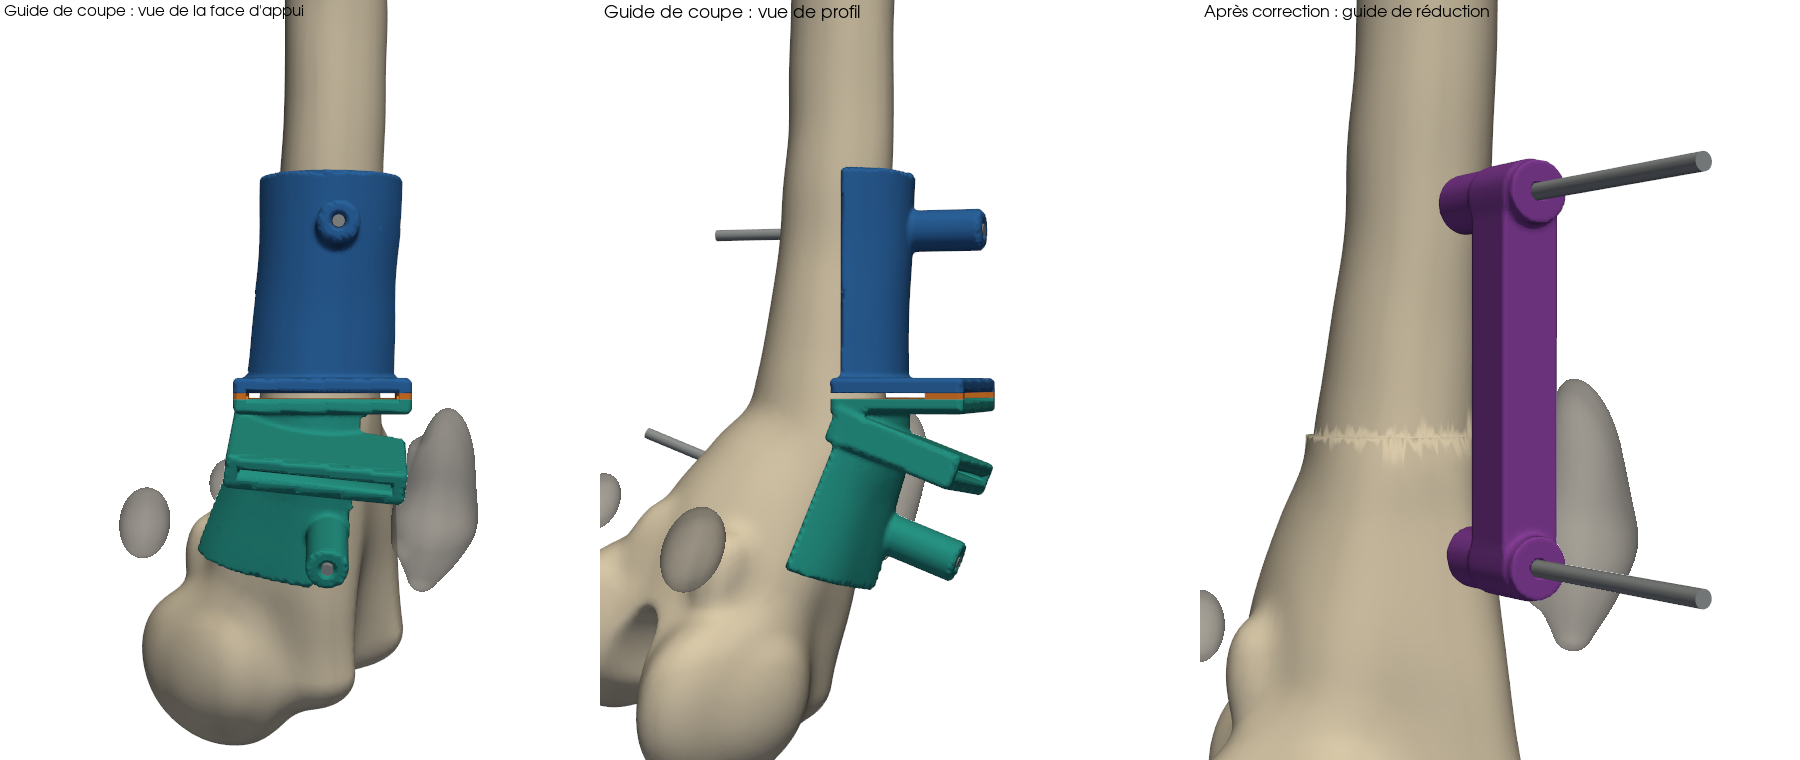
\includegraphics[width=\textwidth]{images/guide_os_fictif.png}\par\vspace{0.3cm}
  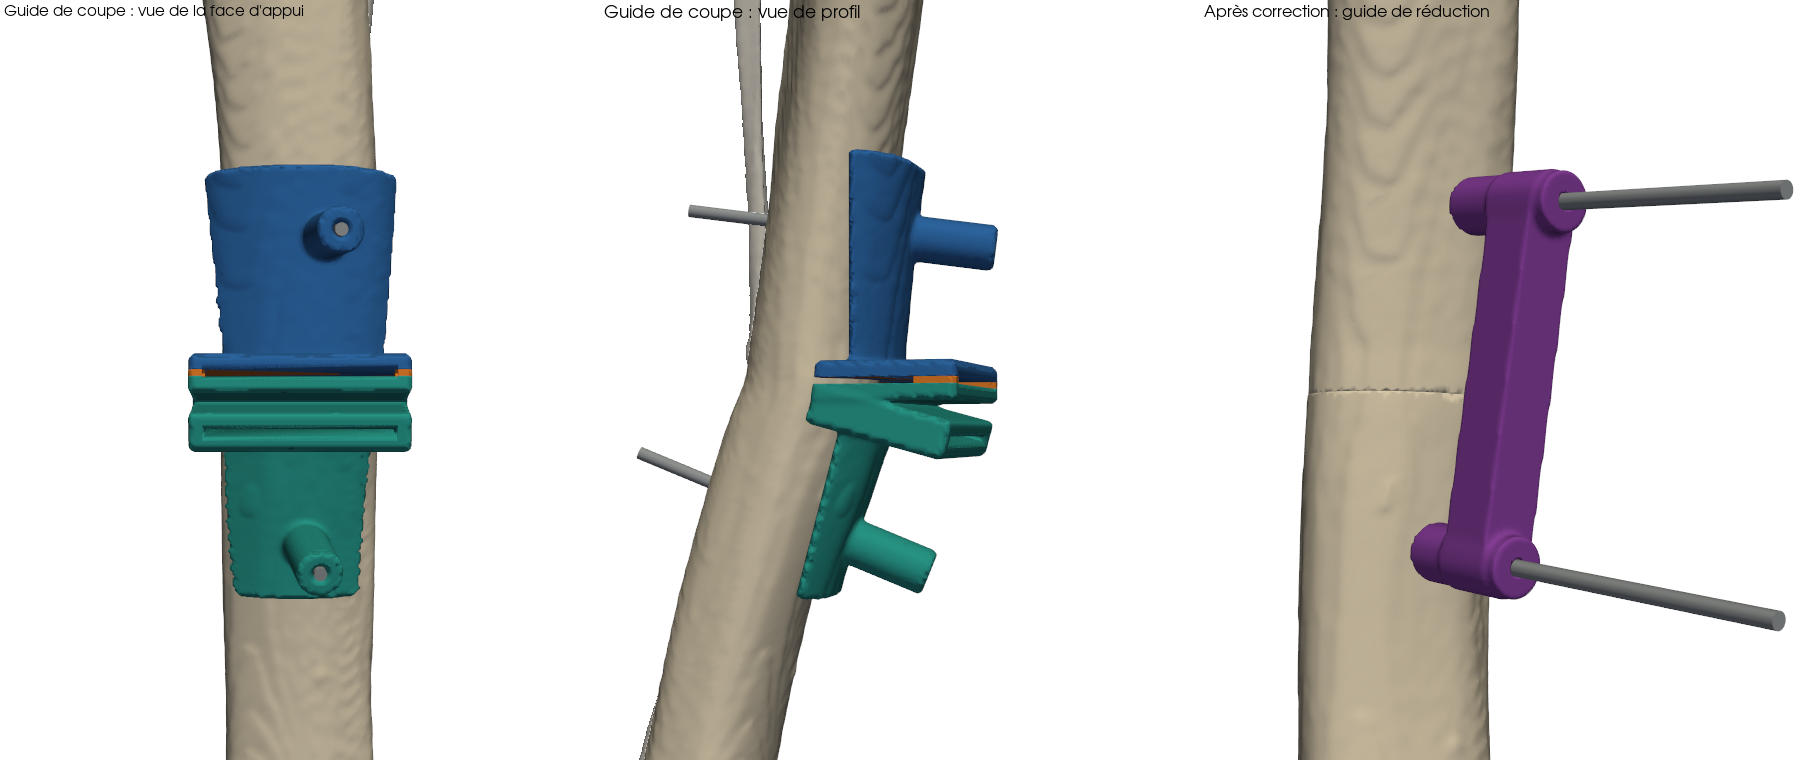
\includegraphics[width=\textwidth]{images/guide_levrier.png}
  \caption{Le même modèle générique adapté à deux os : en haut, le fémur de l'os fictif (coin de fermeture) ; en bas,
  le tibia du lévrier (coin de fermeture). Guide de coupe en bleu et vert, guide de réduction en violet, une broche par
  fragment.}
  \label{fig:guides}
\end{figure}

\section{Limites}

\begin{itemize}
  \item Aucune dimension n'a encore été vérifiée sur une pièce imprimée. Les jeux (fente, manchons) et la tenue des
        ponts doivent être mesurés sur des pièces d'essai en PA12 avant toute utilisation.
  \item L'os fictif est calibré sur un Labrador et le lévrier est un seul chien sain : d'autres races et de vrais os
        déformés restent à essayer.
  \item CT-CORA3D est un prototype de recherche : toute planification doit être validée par un vétérinaire.
\end{itemize}

\end{document}
